% -*- TeX:SI -*-
% slovene sub-mode for spell check
% ----------------------------------------------------------------------
%  Predloga za obliko in navodila za pisanje diplomskih nalog v LaTex-u

%  Univerza v Ljubljani, Fakulteta za elektrotehniko

%  zbral in uredil Roman Kamnik, junij 2013

% ----------------------------------------------------------------------

\documentclass[a4paper,twoside,openright,12pt]{book}
\usepackage[cp1250]{inputenc}  %Kodna stran za Windows okolje, za linux je kodna stran latin2
\usepackage[slovene]{babel}    % pravila za slovensko deljenje besed
\usepackage[pdftex]{UNI-LJ-FE-Diploma} %Stil za diplome na Fakulteti za elektrotehniko (za pdfTeX v MkiTex)
%\usepackage[pctex]{UNI-LJ-FE-Diploma} %Stil za diplome na Fakulteti za elektrotehniko  (za pcTex)
\usepackage{graphicx}

\usepackage{tikz}
\usetikzlibrary{calc}
\usepackage{subcaption} 


\usepackage{hyperref}


\newcommand{\magnet}[5]{% xsredisce, ysredisce, zasuk besedilo v srediscu najb bo crta ali ne
 \pgfmathsetmacro{\Cosa}{cos(#3)}
 \pgfmathsetmacro{\Sina}{sin(#3)}
\draw (#1,#2) circle (2);
\draw (#1+ -2.0 *#5* \Cosa  ,#2 -2.0 *#5* \Sina )--(#1+2.0 *#5* \Cosa , #2+2.0 *#5* \Sina );
\node at (#1-1.6*\Sina ,#2+1.6*\Cosa ){\rotatebox{#3}{N}};
\node at (#1+1.6*\Sina ,#2-1.6*\Cosa  ){\rotatebox{#3}{S}};
\fill (#1,#2) circle [radius=1pt];
}


\newcommand{\senzorja}[4]{% xsredisce, ysredisce, zasuk
 \pgfmathsetmacro{\Cosb}{cos(#3)}
 \pgfmathsetmacro{\Sinb}{sin(#3)}



\hall{#1+2.4*\Cosb }{#2+2.4*\Sinb }{#3}
\hall{#1-2.4*\Sinb}{#2+2.4*\Cosb}{#3}
\fill (#1,#2) circle [radius=1pt];

\draw [dashed, thick](#1,#2)--(#1+2.2*\Cosb ,#2+2.2*\Sinb );
\draw [dashed, thick](#1,#2)--(#1-2.2*\Sinb ,#2+2.2*\Cosb );
}

\newcommand{\hall}[3]{

 \pgfmathsetmacro{\Cosd}{cos(#3)}
 \pgfmathsetmacro{\Sind}{sin(#3)}
 
\draw 
(#1 - 0.2 * \Sind -0.2 * \Cosd  ,#2 + 0.2 * \Cosd -0.2 *\Sind )--
(#1 - 0.2 * \Sind +0.2 * \Cosd  ,#2 + 0.2 * \Cosd +0.2 *\Sind )--
(#1 + 0.2 * \Sind +0.2 * \Cosd  ,#2 - 0.2 * \Cosd +0.2 *\Sind )--
(#1 + 0.2 * \Sind -0.2 * \Cosd  ,#2 - 0.2 * \Cosd -0.2 *\Sind )--
(#1 - 0.2 * \Sind -0.2 * \Cosd  ,#2 + 0.2 * \Cosd -0.2 *\Sind );

\draw (#1-0.1*\Cosd -0.1*\Sind,#2+0.1*\Cosd-0.1*\Sind) --(#1+0.1*\Cosd +0.1*\Sind,#2-0.1*\Cosd+0.1*\Sind);
\draw (#1+0.1*\Cosd -0.1*\Sind,#2+0.1*\Cosd+0.1*\Sind)-- (#1-0.1*\Cosd +0.1*\Sind,#2-0.1*\Cosd-0.1*\Sind);
}
\newcommand{\CaCS}[3]{% razdalja od izhodisca do x max, x komponenta izhodisca, y komponenta izhodisca
	
	\draw [<->](-#1+#2,#3)--(#1+#2,0+#3) node[anchor=north]{$x$};
	\draw [<->](#2,-#1+#3)--(0+#2,#1+#3) node[anchor=east]{$y$};
	
	}

%*************************** PRILAGODITVE *****************************
% mapa s slikami
\potgrafike{./Slike/}
%prilagoditev levega roba sodih strani. �e se pri dvostranskem tisku robovi ne umemajo se lahko pove�a ali pomanj�a
\zamaknirobsodihstrani{0mm}

%*************************** NASLOVNA STRAN *****************************
\naslov{Vpliv stat�ne in dinami�ne ekscentri�nosti na napako senzorja RM44, u�inkovitost kalibracije in robustnost kalibracije na harmonske oscilacije mehanske hitrosti}
\avtor{Mitja Ali�} \univerza{Univerza v Ljubljani}
\fakulteta{Fakulteta za elektrotehniko}
\delo{Magistrsko delo}
%\delo{Diplomsko delo visoko�olskega strokovnega �tudija}
\date{Ljubljana, 2017}
\mentor{doc. dr. Mitja Nemec}
%\somentor{prof. dr. Ime Priimek}
\begin{document}

%------------------------ ZA�ETNI DEL -----------------------------------
%\frontmatter
%%------------------------------------------------------------------------
%
%
%%************************ NASLOVNA STRAN ********************************
%\maketitle
%
%
%%*************************** ZAHVALA ************************************
%\zahvala V zahvali se kandidati zahvali mentorju in poimensko tudi
%vsem sodelavcem in prijateljem, ki so pomagali in prispevali pri
%delu v laboratoriju, na ra�unalniku, v delavnici, pri tehni�ni
%izdelavi dela in drugje.
%
%
%%*************************** VSEBINA *************************************
%\tableofcontents
%
%%*************************** SEZNAM SLIK in TABEL  ***********************
%\seznamslik
%\seznamtabel
%
%%***************************  SEZNAM UPORABLJENIH SIMBOLOV  **************
%
%\seznamsimbolov
%
%V pri�ujo�em zaklju�nem delu so uporabljeni naslednje veli�ine in
%simboli:
%
%\begin{table}[h]
%\centering
%%\begin{footnotesize}
%\begin{tabular}{l l l l}
% \hline \multicolumn{2}{c}{\bf{Veli�ina / oznaka}} & \multicolumn{2}{c}{\bf{Enota}}  \\
% \hline
%Ime & Simbol & Ime & Simbol \\
% \hline
% �as & $t$  & sekunda & s \\
% frekvenca & $f$  & Hertz & Hz \\
% tlak & $p$  & Pascal & Pa \\
% sila vzgona & $\textbf{\textit{f}}_\text{vz}$  & Newton & N \\
% gostota & $\rho$  & - & kg/m$^3$ \\
% masa telesa  & $m_\text{t}$  & kilogram & kg \\
% vhodna napestost & $U_\text{vh}$ & volt  & V \\
% Jacobijeva matrika & $\mathbf{J}$  & - & - \\
%  \hline
%\end{tabular}
%%\end{footnotesize}
%  \caption{Veli�ine in simboli}
%  \label{prebojne_trdnosti}
%\end{table}
%
%
%
%%------------------------ GLAVNI DEL ------------------------------------
%\mainmatter
%%-------------------------------------------------------------------------
%
%
%%********************* POVZETEK V SLOVEN��INI ****************************
%\povzetek
%
%V pri�ujo�em delu so predstavljena navodila za izdelavo 
%
%\kljucnebesede beseda1, beseda2, beseda3
%
%
%%*************************** POVZETEK V ANGLE��INI ***********************
%\abstract
%
%The thesis addresses ...
%
%\keywords word1, word2, word3
%
%
%%***************************** UVOD **************************************
%\chapter{Uvod} \label{uvod}
%
%Uvod v zaklju�no delo ima namen, da uvede bralca v tematiko
%zaklju�nega dela. V njem kandidat raz�leni zahteve in cilje
%zaklju�nega dela, po literaturi povzame znane 
%re"sitve in oceni
%njihov pomen za zaklju�no delo. Sklicevanje na literaturo se v
%besedilu ozna�i s "stevilko v oglatem oklepaju, ki jo ima ta v
%seznamu uporabljenih virov, in po potrebi navede strani, npr.
%\cite{miklavvcivc2010objavljanje} ali \cite[stran 520 -
%534]{juvznivc1992diplomska}.
%
%%*********************** OSREDNJA POGLAVJA ********************************
%\chapter{Izbira teme zaklju�nega dela} \label{izbira_teme}
%
%\chapter{Princip delovanja senzorja RM44}
%
%
%
%
%\chapter{Dolo"canje napake s simulacijo}


\chapter{Uvod}

V dana"snjem "casu elektromotorski pogoni vse hitreje nadome"scajo druge oblike ustvarjanja mehanskega dela. Zahteve po "cim hitrej"si regulaciji in zaneslivosti pogona so "cedalje vi"sje. V pogonih se "zeli dose"ci tudi "cim vi"sji izkoristek. Za doseganje uspe"snega obratovanja elektromotorskega pogona se potrebuje dober in zanesljiv dajalnik pozicije. 
Dejalnike delimo na linearne dajalnike in dajalnike zasuka oz. rotacije. Tu se bom osredoto"cil na rotacijske dajalnike pozicije. Ti so lahko montirani na poljubnem mestu na osi (angl.: through hole), ali le na koncu osi (ang.: On-axis).

%analogni-digitalni senzorji
%relativni absolutni dajalniki

Vsak dajalnik ima to"cnost, katero dose"ze, "ce je pravilno montiran. naapka nepravilne montaze je odvisna od nepravilno postavljenega aktuatorja na osi pogona, ali nepravilno montiranega senzorja. V tem delu bom analiziral kako se napaka ....

V tem delu se bom osredoto"cil na dajalnik RM44, ki ga bom namerno 



Dajalnike lo"cimo tudi glede na uporabljen princip zaznavanja premika. Poznamo magnetne, opti"cne, induktivne in druge. 
Dejalniki se razlikujejo tudi na izodne signale.




\chapter{Dajalniki pozicije RM44}

Dajalnik pozicije RM44 je produkt podjetja RLS merilna tehnika d.o.o. kratica RLS pomeni rotacijski in linearni senzorji zasuka (ang.: Rotary and Linear motion Sensors). Podjetje proizvaja merilnike na podlagi merjenja magnetnega polja. Dajalnik pozicije RM44 spada v dru"zio enkoderjev montiranih na koncu osi rotirajo"ce gredi (ang.: On-axis). Na rotirajo"co os je pritrjen cilindri"cni magnet, ki je diametralno magnetiziran. %(dodaj sliko iz diplome barbare na strani 22 )
Senzor je sestavljen iz "cipa AM8192B, v katerem so vgrajene Hallove sonde za merjenje pravokotne komponente magnetnega polja, magneta montiranega na os pogona. Izhod senzorja je lahko analogen v obliki dveh signalov sinusa in kosinusa. Izhod senzorja je lahko inkrementalni, ki poda relativno spremembo pozicije ter smer premikanja. Senzor lahko prika"ze tudi absolutno vrednost pozicije. Njegova resolucija je nastavljiva med 320 in 8192 pozicij na obrat.

\chapter{Analiti"cna izpeljava dinami"cne in stati"cne eks"centri"cnosti}

Napake so prisotne pravzaprav pri vsakem senzorju. V tem poglavju bom analiti"cno prikazal vpliv napak omenjenih ekscentri"cnosti, ki se pojavijo ob nepravilni monta"zi senzorja. Njuna vpliva ra"zli"cno vplivata na napako zato ju bom obravnaval posami"cno. V delu sem predpostavil, da se izmiki iz idealne pozicije izmikajo le v smeri x in y. Napaka se pojavi tudi ob premiku v smeri z vendar tega tu nebom obravnaval.
 Zaradi narave problema je smiselno uporabiti kartezi"ni koordinatni sistem. V izpeljavah bom predpostavil, da so izmiki majhni. Najprej bom izpeljal po ka"sni trajetoriji se giblje posamezna Hallova sonda. Iz znane tretnutne lokacije Hallove sonde bom lahko izra"cunal vrednost B komponente ki jo meri posamezna Hallova sonda. Pri analiti"cni izpeljavi bom predopstavil, da je polje ob majhnih odmikih linearno in ustreza enacbi polja $B(x,y)=k \cdot y$.  Nato bom analiti"cno izrazil vrednost kota, ki predstavlja izhod senzorja.



\section{Za"cetna pozicija senzorjev}

Za dolo"canje kota med vektorjem ki ka"ze v smeri x-os (\textbf{$1_x$}) in vektorjem med koordinatnim izhodiscem in poljubno to"cko v koordinatnem sistemu, je potrebno poznati poznati le polo"zaj to"cke. Primer je podan na sliki \ref{fig:dolocitev_kota}. Kot $\varphi$ dolo"cimo preko trigonometri"cne funkcije $\arctan$: $$\varphi=\arctan\frac{y_0}{x_0}$$



\begin{figure}[h!]
	\centering
	\begin{tikzpicture}[scale=4]
	\CaCS{0.75}{0}{0}
	\draw [->,thick](0,0)--(-0.5,0.2855);
	\draw (0.15,0) arc (0:150:0.15);
	\node at (0.05,0.05){$\varphi$};
%	\node at (-0.5,0.285) {\textbullet};
	\node at (-0.32,0.35) {($x_0$,$y_0$)};
	\end{tikzpicture}
	\caption{Slika za pomo"c pri dolo"canju kota}
	\label{fig:dolocitev_kota}
\end{figure}


Za dolo"citev kota $\varphi$  je dovolj poznati "ze projekciji vektorja na koordinatni osi(slika \ref{fig:dolocitev_kota_2}),

\begin{figure}[h!]
	\centering
	\begin{tikzpicture}[scale=4]
	\CaCS{0.75}{0}{0}
	\draw [->,thick](0,0)--(-0.5,0.2855);
	\draw (0.15,0) arc (0:150:0.15);
	\node at (0.05,0.05){$\varphi$};
	\draw [dashed] (-0.5,0.2855)--(-0.5,0);
	\draw [dashed] (-0.5,0.2855)--(0,0.2855);
	%	\node at (-0.5,0.285) {\textbullet};
%	\node at (-0.32,0.35) {($x_0$,$y_0$)};
	\node at(-0.5,-0.1){$x_0$} ;
	\node at(0.1,0.2855){$y_0$};
	\end{tikzpicture}
	\caption{Slika za pomo"c pri dolo"canju kota}
	\label{fig:dolocitev_kota_2}
\end{figure}


"Ce poznamo le projekciji to"cke na koordinatni osi, je to zadosten pogoj za dolo"citev kota $\varphi$.
Za dolo"citev kota zasuka v idealnih pogojih, kot je predpostavka, da je polje linearno, sta dovolj dve Hallovi sondi, ki sta prostorsko zamaknjeni za 90$^\circ$ (Slika \ref{fig:zacetna_postavitev_sond}).

Za"cetni lokaciji sond enostavmo postavimo na koordinatni osi in s tem ustre"zemo pogoju po prostorskem zasuku med sondama. Sondi postavimo na razdaljo $r_0$ od koordinatnega izhodi"s"ca. S tem dobimo za"cetni lokaciji Hallovih sond $\mathrm{H}_1(x_0, y_0)=(r_0, 0)$, $\mathrm{H}_2(x_0, y_0)=(0, r_0)$.



\begin{figure}[h!]
	\centering
	\begin{tikzpicture}[scale=1]
	\CaCS{3}{0}{0}
	\senzorja{0}{0}{0}{}
%	\magnet {0} {0} {10}{ }{0}
	\node at (2.0,-0.5){$\mathrm{H}_1(r_0,0)$};
	\node at (-1,2.3){$\mathrm{H}_2(0, r_0)$};
	\end{tikzpicture}
	\caption{Za"cetna postavitev Hallovih sond}
	\label{fig:zacetna_postavitev_sond}
\end{figure}


\section{Zasuk magneta}

Z zasukom magneta za kot $\theta$ se na mestu, kjer merimo magnetno polje, polje spremni. Polje bi se spremnilo enako "ce bi nad magnetom  zasukali senzor za kot $-\theta$. Hallova sonda z za"cetno lokacijo ($x_0, y_0$) bi se po kro"znici premaknila v novo lokacijo($\mathrm{x, y}$):
\begin{equation}
\label{eq:osnovni_zasuk}
\begin{bmatrix}
x\\y
\end{bmatrix}= \begin{bmatrix}
\cos (-\theta)& -\sin(-\theta)\\ \sin( -\theta)& \cos (-\theta)
\end{bmatrix}
\cdot
\begin{bmatrix}
x_0\\y_0
\end{bmatrix}
\end{equation}
Z upo"stevanjem da je funkcija sinus liha in funkcija kosinus soda, se izra"cun v ena"cbi \ref{eq:osnovni_zasuk} poenostavi v:
\begin{equation}
\label{eq:osnovni_zasuk_popravljena_rot}
\begin{bmatrix}
x\\y
\end{bmatrix}= \begin{bmatrix}
\cos (\theta)& \sin(\theta)\\ -\sin( \theta)& \cos (\theta)
\end{bmatrix}
\cdot
\begin{bmatrix}
x_0\\y_0
\end{bmatrix}
\end{equation}




\begin{figure}[h!]
	\begin{subfigure}[b]{0.5\textwidth}
		\centering
		
		\resizebox{\linewidth}{!}{
			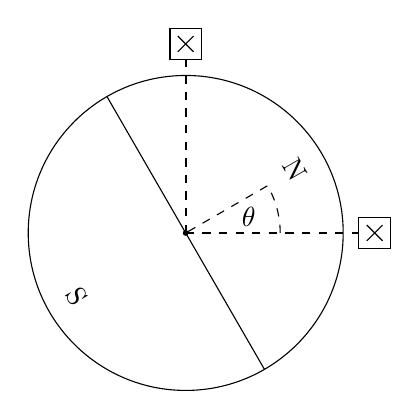
\begin{tikzpicture}
	\senzorja{0}{0}{0}{ }
	\magnet {0} {0} {-60}{ }{1}

	\draw (1.2,0) arc (0:30:1.2) node at (0.8,0.2){$\theta$}[dashed]--(0,0);
			\end{tikzpicture}
		}
		
		\caption{Zasukan magnet za kot $\mathrm{\theta}$}
		\label{fig:subfig8}
	\end{subfigure}
	\begin{subfigure}[b]{0.5\textwidth}
		\centering
		\resizebox{\linewidth}{!}{
			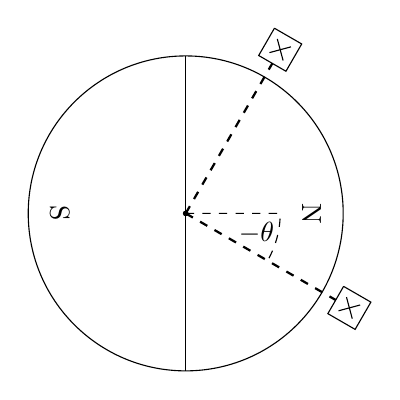
\begin{tikzpicture}

				\senzorja{0}{0}{-30}{ }
				\magnet {0} {0} {-90}{ }{1}
				\draw [dashed](0,0)--(1.2,0) arc (0:-30:1.2);
				\node at (0.9,-0.25){$-\theta$};
			\end{tikzpicture}
		}
		\caption{Zasukan senzor za kot $\mathrm{-\theta}$}   
		\label{fig:subfig9}
	\end{subfigure}

	\caption{Hallovi sondi se glede na magnet nahajati na enaki lokaciji}
	\label{fig:subfig1.a.4}
\end{figure}




Ko zavrtimo senzor okoli magneta pri tem pomeri polje. Ker sem predpostavil linearno polje, ga predstavim s izrazom 
\begin{equation}
\label{eq:enacba_polja}
B(x,y)=k \cdot x
\end{equation}
Za poenostavitev vzemimo $k=1$. S tem se ena"cba \ref{eq:enacba_polja} poenostavi v:
\begin{equation}
\label{eq:enacba_polja_2}
B(x,y)=x
\end{equation}


Polje ki ga pomeri posamezna sonda dobimo z upostevanjem ena"cb \ref{eq:osnovni_zasuk_popravljena_rot} in \ref{eq:enacba_polja_2}.
\begin{equation}
B_{H_1}(\theta)=r_0\cdot \sin \theta
\end{equation}
\begin{equation}
B_{H_2}(\theta)=r_0\cdot \cos \theta
\end{equation}

\slikaeps{Magnetno polje, ki ga pomeriti sondi, ko je monta"za pravilna}{B1B2_brez_eks}


\section{Izpeljava ena"cb pri dinami"cni ekscentri"cnosti}

%Zaradi splo"snosti predpostavimo da sta sredi"s"ci v za"cetni legi poravnani vendar je magnet glede na senzor zasukan za kot $\lambda$ (Slika \ref{fig:definicija_lambde}).  Ta je v primeru ko je smer poravnana z za"cetno lego magneta enaka 0. V nasprotnem primeru pa kot upo"stevamo v definiciji njene lege glede na kot magneta $\theta -\lambda$.  Ta zasuk bo imel na obe Hallovi sondi enak vpliv. Zato si lahko privo"s"cimo implementacijo kota  $\lambda$, ki temelji na principu superpozicije. 
%
%
%\begin{figure}[h!]
%	\centering
%	
%	\begin{tikzpicture}
%	\senzorja{0}{0}{0}{ }
%	\magnet {0} {0} {-60}{ }{1}
%	
%	\draw[dashed](0.0,0)--(1.5,0)arc(0:30:1.5)--(0.,0);
%	\node at (1.2,0.3){$\lambda$};
%	
%	\end{tikzpicture}
%	
%	\caption{Zasukan magnet za kot $\mathrm{\theta}$}
%	\label{fig:definicija_lambde}
%	
%\end{figure}
Opazujmo sedaj opisan sistem z dodano dinami"cno ekscentri"cnostjo. Definirajmo za"cetno lego rotorja v centru statorja $S_r(0, 0)=S_s(0, 0)$. Rotor izmaknemo iz za"cetne lege v novo sredi"s"ce $S_r(\Delta x_d, \Delta y_d,)$. Os vrtenja ostaja v centru statorja, zato staro sredi"s"ce rotorja opisuje kro"znico s polmerom $\sqrt{\Delta x_d^2+ \Delta y_d^2}$. 






\begin{figure}[h!]
	\begin{subfigure}[b]{0.5\textwidth}
		\centering
		\resizebox{\linewidth}{!}{
			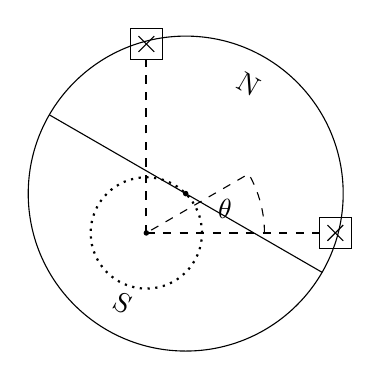
\begin{tikzpicture}
	\senzorja{0}{0}{0}{$S_s(0, 0)$}
	\magnet {0.5} {0.5} {-30}{$S_r(\Delta x_d, \Delta y_d)$}{1}
	\draw [dotted,thick](0,0) circle [radius=0.707];
	\draw [dashed](1.5,0) arc (0:30:1.5)--(0,0);
	\node at(1,0.3){$\theta$};
			\end{tikzpicture}
		}
		\caption{Zasukan magnet za kot $\mathrm{\theta}$}
		\label{fig:teorija_dinamika_1}
	\end{subfigure}
	\begin{subfigure}[b]{0.5\textwidth}
		\centering
		\resizebox{\linewidth}{!}{
			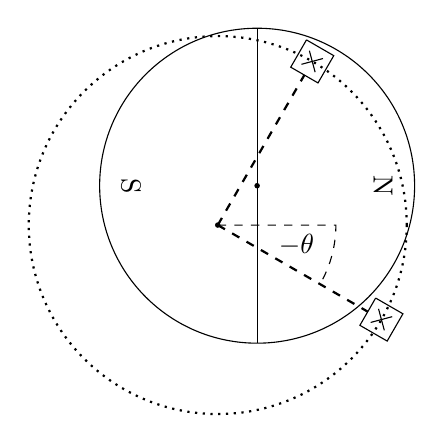
\begin{tikzpicture}
	\senzorja{-0.5}{-0.5}{-30}{$S_s(-\Delta x_d, -\Delta y_d)$}
	\magnet {0} {0} {-90}{$S_r(0, 0)$}{1}
	\draw [dotted, thick](-0.5, -0.5) circle [radius=2.4];
	
	\draw  [dashed](-0.5,-0.5)--(1,-0.5) arc (0:-30:1.5);
	\node at (0.5, -0.75){$-\theta$};
			\end{tikzpicture}
		}
		\caption{Zasukan senzor za kot $\mathrm{-\theta}$}   
		\label{fig:teorija_dinamika_2}
	\end{subfigure}ub
	
	\caption{Hallovi sondi se glede na magnet nahajati na enaki lokaciji}
	\label{fig:subfig1.a.4}
\end{figure}




"Ce sedaj sistem miselno obrnemo kot sem to napravil v prej"njem poglavju in senzor zavrtimo. Ob takem premiku senzor opi"se trajektorijo kot pri pravilno montiranem senzorju le z dodano translacijo ekscentri"cnosti. Kako Hallova sonda spreminja lokacijo glede na vrtenje je prikazano na sliki \ref{fig:teorija_dinamika_2}, s pik"casto kro"znico.


Novo lokacijo Hallove sonde lahko dolo"cimo po ena"cbi \ref{eq:dinamicna_ekscentricnost}.
\begin{equation}
\label{eq:dinamicna_ekscentricnost}
\begin{bmatrix}
x\\y
\end{bmatrix}= \begin{bmatrix}
\cos (\theta)& \sin(\theta)\\ -\sin( \theta)& \cos (\theta)
\end{bmatrix}
\cdot
\begin{bmatrix}
x_0\\y_0
\end{bmatrix}
+
\begin{bmatrix}
-\Delta x_d \\ -\Delta y_d
\end{bmatrix}
\end{equation}
Ena"cbo \ref{eq:dinamicna_ekscentricnost} lahko poenostavimo pri "cemer $\Delta x_d$ in $\Delta y_d$ predstavlja vrednost za koliko je rotor izmaknjen iz osi vrtenja.
\begin{equation}
\label{eq:dinamicna_ekscentricnost_popravljena}
\begin{bmatrix}
x\\y
\end{bmatrix}= \begin{bmatrix}
\cos (\theta)& \sin(\theta)\\ -\sin( \theta)& \cos (\theta)
\end{bmatrix}
\cdot
\begin{bmatrix}
x_0\\y_0
\end{bmatrix}
-
\begin{bmatrix}
\Delta x_d \\ \Delta y_d
\end{bmatrix}
\end{equation}

Z upo"stevanjem magnetnega polja po izrazu \ref{eq:enacba_polja_2} izrazimo odvistnost magnetnega polja od kota zasuke in ekscenri"cnosti. Iz potekov magnetnega polja v izrazih (\ref{eq:B_H_1_dinamicen}) in (\ref{eq:B_H_2_dinamicen}) opazimo da magnetno polje ni odvisno od dinami"cne eks"centri"cnosti v y smeri. S hitrim miselnim eksperimentom si lahko hitro predstavljamo, da "ce senzor izmaknemo v smeri y magnetno polje na novi lokaciji ostane enako. 

\begin{equation}
\label{eq:B_H_1_dinamicen}
B_{H_1}(\theta)=r_0\cdot \cos \theta -\Delta x_d
\end{equation}
\begin{equation}
\label{eq:B_H_2_dinamicen}
B_{H_2}(\theta)=r_0\cdot \sin \theta-\Delta x_d
\end{equation}



\slikaeps{Magnetno polje, ki ga pomeriti sondi, ko je magnet izmaknjen}{B1B2_din_eks}





\section{Izpeljava ena"cb pri stati"cni ekscentri"cnosti}

Opazovani sistem ostaja enak, brez ekscentri"cnosti. Sedaj iz osi vrtenja izmaknemo senzor. Os magneta in os vrtenja sta poravnani.  Sredi"s"ce senzorja se sedaj nahaja na koorinatah $S_s(\Delta x_s, \Delta y_s)$. kot pri izpeljavi pri dinami"cni ekscentri"cnosti obrnimo sistem in zavrtimo senzor upo"stevajo"ce z ekscentri"cnostjo. Sredi"s"ce senzorja opi"se kro"znico okoli sredi"sca magneta oz. osi vrtenja. Hallovi sondi se vrtita vsaka po svoji kro"znici. Gibanje posamezne sonde lahko opi"semo z izrazom:

   \begin{equation}
   \label{eq:dinamicna_ekscentricnost_popravljena}
   \begin{bmatrix}
   x\\y
   \end{bmatrix}=
   \begin{bmatrix}
   \cos (\theta)& \sin(\theta)\\ -\sin( \theta)& \cos (\theta)
   \end{bmatrix}
   \cdot
   \begin{bmatrix}
   x_0+\Delta x_s\\y_0+\Delta y_s
   \end{bmatrix}
   \end{equation}

Magnetno polje, ki ga pomerita dobimo iz izraza (\ref{eq:enacba_polja_2}).

\begin{equation}
\label{eq:B_H_1_staticen}
B_{H_1}=(r_0+\Delta x_s)\cos(\theta)+\Delta y_s \sin(\theta)
\end{equation}
\begin{equation}
\label{eq:B_H_2_staticen}
B_{H_1}=-\Delta x_s\sin(\theta)+(r_0+\Delta y_s) \cos(\theta)
\end{equation}













\begin{figure}[h!]
	\begin{subfigure}[b]{0.5\textwidth}
		\centering
		\resizebox{\linewidth}{!}{
			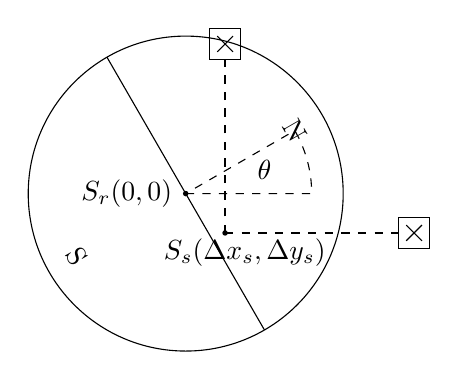
\begin{tikzpicture}
			\senzorja{0.5}{-0.5}{0}{$S_s(\Delta x_s, \Delta y_s)$}
			\magnet {0} {0} {-60}{$S_r(0, 0)$}{1}
		
		
			\node at (0.75,-0.75){$S_s(\Delta x_s, \Delta y_s)$};
			\node at (-0.75,0){$S_r(0, 0)$};
			
		
			\draw [dashed](0,0)--(1.6,0) arc (0:30:1.6)--(0,0);
			\node at(1,0.3){$\theta$};
			

			
			\end{tikzpicture}
		}
		\caption{Zasukan magnet za kot $\mathrm{\theta}$ in statina eksenri"cnost}
		\label{fig:teorija_statika_1}
	\end{subfigure}
	\begin{subfigure}[b]{0.5\textwidth}
		\centering
		\resizebox{\linewidth}{!}{
			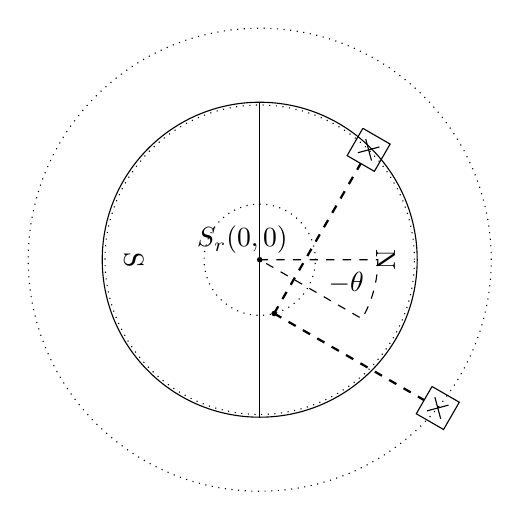
\begin{tikzpicture}
%			\senzorja{0.5}{-0.5}{0}{$S_s(-\Delta x_d, -\Delta y_d)$}
			\senzorja{0.183}{-0.683}{-30}{$S_s(-\Delta x_d, -\Delta y_d)$}
			\magnet {0} {0} {-90}{$S_r(0, 0)$}{1}


			\draw [dashed](0,0)--(1.5,0) arc (0:-30:1.5)--(0,0);
			\node at(1.1,-0.3){$-\theta$};


			
			
			\draw [dotted](0,0) circle [radius=0.707];
		
%			\node at (0,-1){$S_s(\Delta x_s, \Delta y_s)$};
			\node at (-0.22,0.25){$S_r(0, 0)$};			
		
     			\draw [dotted](0,0) circle	[radius=2.94];
     			\draw [dotted](0,0) circle	[radius=1.965];
     		                                                                                     
			\end{tikzpicture}
		}
		\caption{Zasukan senzor za kot $\mathrm{-\theta}$}   
		\label{fig:teorija_statika_2}
	\end{subfigure}ub
	
	\caption{Hallovi sondi se glede na magnet nahajati na enaki lokaciji}
	\label{fig:subfig1.a.4}
\end{figure}




\slikaeps{Magnetno polje, ki ga pomeriti sondi, ko je senzor izmaknjen}{B1B2_sta_eks}


\section{Kon"cna ena"cba za dolo"citev lokacije sonde in dolo"canje pomerjenega kota}


Sedaj lahko izraza za dolo"canje lokacije in hkrati magnetnega polja zapi"semo z eno ena"cbo:



   \begin{equation}
   \label{eq:enacba_lokacije}
   \begin{bmatrix}
   x\\y
   \end{bmatrix}=
   \begin{bmatrix}
   \cos (\theta)& \sin(\theta)\\ -\sin( \theta)& \cos (\theta)
   \end{bmatrix}
   \cdot
   \begin{bmatrix}
   x_0+\Delta x_s\\y_0+\Delta y_s
   \end{bmatrix}
   -
   \begin{bmatrix}
   \Delta x_d\\ \Delta y_d
   \end{bmatrix}
   \end{equation}

Polje ki ga opi"seti sondi se glasi:
\begin{equation}
\label{B_H_1_koncna}
B_{H_1}=(r_0+\Delta x_s) \cos(\theta)+\Delta y_s \sin(\theta)-\Delta x_d
\end{equation}
\begin{equation}
\label{B_H_2_koncna}
B_{H_2}=\Delta x_s \cos(\theta)+(r_0+\Delta y_s) \sin(\theta)-\Delta x_d
\end{equation}

Iz izrazov (\ref{B_H_1_koncna}) in (\ref{B_H_2_koncna}) sedaj lahko izra"cunamo kot.

\begin{equation}
\label{eq:dolocanje_kota_splosna}
\varphi=\arctan \frac{B_{H_2}}{B_{H_1}}
	=\arctan \frac{\Delta x_s \cos(\theta)+(r_0+\Delta y_s) \sin(\theta)-\Delta x_d}
	{(r_0+\Delta x_s) \cos(\theta)+\Delta y_s \sin(\theta)-\Delta x_d}
\end{equation}


%https://dspguru.com/files/Sum_of_Two_Sinusoids.pdf vir za izracun trigonometrije


%http://ieeexplore.ieee.org/stamp/stamp.jsp?arnumber=6375931
%http://ieeexplore.ieee.org/stamp/stamp.jsp?arnumber=6567733
%http://ieeexplore.ieee.org/stamp/stamp.jsp?arnumber=4054743
%http://ieeexplore.ieee.org/stamp/stamp.jsp?arnumber=5346438
%http://www.embedded.com/design/other/4216719/Performing-efficient-arctangent-approximation
%

%Zaradi majhnih odmikov lahko predpostavim, da je pravokotna komponenta vektorja gostote magnetnega pretoka(vektor \textbf{B}) linearna. S tem se izpeljava za dolo"canje pozicije, poenostavi. Kasneje bom predstavil tudi na"cin kako pridobiti vredn ost \textbf{B} realnega polja. Predpostavil bom tudi da je senzor za mejenje pozicije sestavljen le iz dveh Hallovih sond, pri kateri je druga sonda fazno premaknjena za 90$^\circ$. 
%slika kjer je narisano linearno polje

\section{Dolo"canje kota pri stati"cni ekscntri"cnosti v smeri x }

Zaradi nelinearnosti fukcije $\arctan$ je izraz (\ref{eq:dolocanje_kota_splosna}) analiti"cno te"zko poenostaviti v polni obliki. Zato se vsake ekscentri"cnosti lotim posami"cno. "Ce upo"stevamo le ekscentri"cnost $\Delta x_s$ se izraz (\ref{eq:dolocanje_kota_splosna}) poenostavi v:
\begin{equation}
\label{eq:dolocanje_kota_xs}
\varphi=
\arctan \frac{\Delta x_s \cos(\theta)+r_0 \sin(\theta)}
{(r_0+\Delta x_s) \cos(\theta)}
\end{equation}


Z upo"stevanjem Taylorjeve vrse za $\arctan$:
\begin{equation}
\arctan(x)=x-\frac{x^3}{3}... pri |x|\leq 1
\end{equation}

Izraz lahko zapi"semo kot

\begin{equation}
\varphi=  \frac{\Delta x_s \cos(\theta)+r_0 \sin(\theta)}
{(r_0+\Delta x_s) \cos(\theta)}+
\frac{(\Delta x_s \cos(\theta)+r_0 \sin(\theta))^3}
{3((r_0+\Delta x_s) \cos(\theta))^3}
\end{equation}



\section{Dolo"canje pribli"zka za funkcijo $\arctan$}

Funkcija arkustangens ($\arctan$), je inverzna funkcija funkcije tangens.

Zaloga vrednosti je v obmo"cju med $-\pi/2$ in $\pi/2$. Funkcija arkustangens tako zajame le polovico periode. V numeriki se za dolo"citev kota na celi periodi
 $[-\pi, \pi]$ uporablja funkcijo $atan2$, ki sprejme dva parametra in na podlagi njunih predznakov dolo"ci v katerem kvadrantu se nahaja iskani kot. 
 
 \[
 \varphi=atan2(x,y)=
 \begin{cases}
 [0, \frac{\pi}{2}]:&  x\geq 0, y\geq 0 \\
 [\frac{\pi}{2}, \pi]:& x\leq 0, y\geq 0\\
 [-\pi, -\frac{\pi}{2}]:& x\leq 0, y\leq 0\\
 [-\frac{\pi}{2}, 0]:& x\geq 0, y\leq 0
 \end{cases}
 \]




Funkcija $atan2$ nato preko funkcije $\arctan$ izra"cuna vrednost na podlagi razmerja $\frac{y}{x}$. Iz izraza (\ref{eq:arctan_picetrt}) lahko vidimo, da je potrebno poznati za funkcijo $\arctan$ zalogo vrednosti le med $-\frac{\pi}{4}$ in $\frac{\pi}{4}$. 
 \begin{equation}
\label{eq:arctan_picetrt}
 \arctan x=\frac{\pi}{2}-\arctan \frac{1}{x}
\end{equation}

Za dolo"citev kota ne glede kje na periodi, je potrebno izra"cunati kvocient med spremenljivko x in y. Da bi se izognil temu deljenju sem aproksimiral funkcijo $f(x,y)=\arctan(\frac{y}{x})$ z ravnino (\ref{eq:polinom}).
\begin{equation}
\label{eq:polinom}
\varphi(x,y)=a_1 x^3 + a_2 x^2 y + a_3 x^2 + a_4 x y^2 + a_5 x y + a_6 x + a_7 y^3 + a_8 y^2 + a_9 y + a_{10}
\end{equation}

Funkcijo sem aproksimiral na naklju"cno razporejene to"cke po "cetrtini kro"znega  kolobarja $\varphi \in [-\frac{\pi}{4}, \frac{\pi}{4}]$, z radijema $a=r_0-0.2$~mm in $b=r_0+0.2$~mm.



\begin{figure}[!h]
	\label{fig:obmocje_tock}
	\centering
	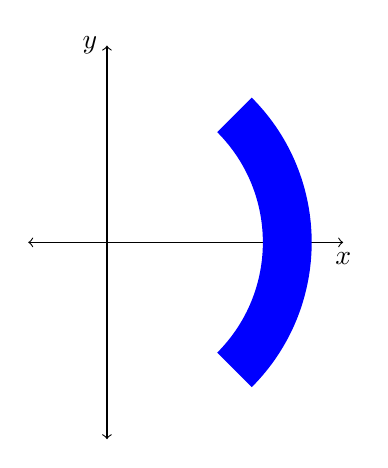
\begin{tikzpicture}
	\draw [<->](-1,0)--(3,0) node[anchor=north]{$x$};
	\draw [<->](0,-2.5)--(0,2.5) node[anchor=east]{$y$};
	\fill [blue] (1.5556*0.9,-1.5556*0.9) arc (-45:45:2.2*0.9)--(1.0*1.8385,1.0*1.8385)arc (45:-45:1.0*2.6)--(1.5556*0.9,-1.5556*0.9);
		\end{tikzpicture}
		\caption{Obmo"cje nahajanja akljucnih to"ck}
\end{figure}

Za to"cke znotraj obmo"cja sem izracunal vrednost $\arctan \frac{y}{x}$. Na to sem z uporabo funkcije polyfitn(dodaj vir), aproksimiral ravnino definirano z izrazom (\ref{eq:polinom}). Dobil sem koeficiente katere sem lahko uporabil v izra"cunih za analiti"cen prikaz napake. Ravnina je na definiranem obmo"cju odstopala za najve"c $0,253^\circ$. S predpostavko, da bo napaka ob dovolj veliki ekscentri"cnosti, vi"sja od napake zaradi aproksimacije ravnine sem v izraz za ravnino, vstavil izraza (\ref{B_H_1_koncna}) in(\ref{B_H_2_koncna}). Izpeljava je prikazana v dodatku. Izrazi se poenostavijo "ce posami"cno obravnavam vsako ekcentri"cnost. 

Z vnosom "stevilk sej je pokazalo, da bo pri stati"cnem izmiku nekoliko bolj izrazit drugi harmonik napake, kot pri dinami"cni ekscentri"cnosti. 

Tu se kaj napisati

Ve"c informacij je bilo te"zko izlu"sciti, saj je bila funkcija $\arctan$ aproksimirana z ravnino dveh spremenljivk le na "cetrtini celotne periode.

\chapter{Numeri"cen izra"cun napake}

Od tu naprej sem za izra"cun kota uporabljal vgrajeno funkcijo $atan2$, ki numeri"cno dolo"ci izhodni kot $\varphi$ glede na vhodni spremenljivki x in y. Pri izra"cunih sem postavil hallovi sondi na razdaljo $r_0=2,4$~mm, vsako ekscentri"cnost posamezno  sem simuliral z $0,1$~mm izmikom.

\subsection{Napaka pri stati"cni ekscentri"cnosti v smeri x-osi}

Z vnosom izrazov (\ref{B_H_1_koncna}) in (\ref{B_H_2_koncna}) v funkcijo $atan2$, s stati"cno ekscentri"cnostjo v x-osi se pojavi napaka definirana kot 
\begin{equation}
\varepsilon= \varphi - \theta
\end{equation}


  \begin{figure}[h!]
  	\begin{center}
  		\includegraphics[scale=0.5]{\dirslike/protokol_xs_1.eps}
  	\end{center}
  	\caption{numericen izracun napake}
  	\label{fig:protokol_xs_1}
  \end{figure}

Iz slike \ref{fig:protokol_xs_1} se vidi napaka v obliki enosmerne komponente in drugega harminika na periodo. Napaka se s konstantnim vrtenjem magneta ne akumulira, zato je dovolj prikaz napake na eni periodi. Napako razvijem v Fouriejevo vrsto do osmega harmonika. Amplitude posameznih harmonikov za stati"cno ekscentri"cnost v smeri x osi za izmik $0,1$~mm so prikazane na sliki \ref{fig:vrsta_protokola_xs_1}.

\begin{figure}[h!]

	\includegraphics[scale=0.7]{\dirslike/vrsta_protokola_xs_1}
	\caption{AAmplitude harmonikov protokola}
	\label{fig:vrsta_protokola_xs_1}
\end{figure}


Kot smo "ze predpostavili po sliki \ref{fig:protokol_xs_1} izstopata predvsem enosmerna komponenta in drugi harmonik. Nakaj je "se "cetrtega harmonika medtem ko so ostali harmoniki zanemarljivi.



\subsection{Napaka pri stati"cni ekscentri"cnosti v smeri y-osi}


Pri stati"cni ekscentri"cnosti sem ponovil postopek kot pri stati"cni ekscentri"cnosti v smeri x-osi. Pri"cakoval sem podobene rezultate, kot pri stati"cni ekscentri"cnosti v smeri x-osi. Napaka kota $\varepsilon$ je prikazana na sliki \ref{fig:protokol_ys_1}. Prav tako kot pri napaki ob stati"cni ekscentri"cnosti v smeri x-osi izstopa enosmerna komponenta in drugi harmonik. Opazimo, da je enosmerna komponenta spremenila predznak. Iz Fouriejeve vrste (slika \ref{fig:vrsta_protokola_ys_1}) Opazimo rezultate podobne kot pri stati"cni ekscentri"cnosti v smeri x-osi. Izstopajo enosmerna komponenta drugi harmonik, obstaja tudi "cetrti harmonik, ostali so zanemarljivi. 
Zanimivost lahko razberemo "se iz faznega premika. Napaka pri stati"cni ekscentri"cnosti v smeri y-osi, za stati"cno napako v smeri x-osi, fazno zaostaja ravno za velikost dveh faznih kotov. To se pojavi pri drugem in "sestem harmoniku. "sesti harmonik je po amplitudi zanemarljiv zato je zanimiv podatek o faznem kotu le za drugi harmonik.


  \begin{figure}[h!]
  	\begin{center}
  		\includegraphics[scale=0.5]{\dirslike/protokol_ys_1.eps}
  	\end{center}
  	\caption{numericen izracun napake}
  	\label{fig:protokol_ys_1}
  \end{figure}
  
  
\begin{figure}
	
	\includegraphics[scale=0.7]{\dirslike/vrsta_protokola_ys_1}
	\caption{AAmplitude harmonikov protokola}
	\label{fig:vrsta_protokola_ys_1}
\end{figure}


\subsection{Napaka pri dinami"cni ekscentri"cnosti v smeri x-osi}
\label{Napaka pri dinami"cni ekscentri"cnosti v smeri x-osi}

"Ze iz analiti"cnih izrazov lahko pri"cakujemo, da bo tu manj"sa izrazitost drugega harmonika. Napaka kota $\varepsilon$ je prikazana na sliki \ref{fig:protokol_xd_1}. Izrazit je predvsem prvi harmonik. Nezanemarljiv je "se drugi harmonik, ostale komponente Fourierjeve vrste pa so zanemarljive.

  \begin{figure}[h!]
  	\begin{center}
  		\includegraphics[scale=0.5]{\dirslike/protokol_xd_1.eps}
  	\end{center}
  	\caption{numericen izracun napake}
  	\label{fig:protokol_xd_1}
  \end{figure}
\begin{figure}
	
	\includegraphics[scale=0.7]{\dirslike/vrsta_protokola_xd_1}
	\caption{AAmplitude harmonikov protokola}
	\label{fig:vrsta_protokola_xd_1}
\end{figure}






\section{Linearno ve"canje napake in opazovanje posameznih harmonikov pogre"ska}


Sedaj poglejmo kako se spreminja posamezna amplituda ekcentri"cnosti glede na velikost ekscentri"costi. Posami"cno sem ve"cal ekscentri"cnosti in pri tem opazoval spreminjanje pogre"ska $\varepsilon$. Pogre"sek $\varepsilon$ sem razvil v fourierovo vrsto in opazoval amplitudo posameznega harmonika $A_n \cos( n \theta)+B_n \sin(n \theta)$.


\subsection{Ve"canje stati"cne napake v x-osi}
Z ve"canjem stati"cne napake se spreminja amplituda posameznih harmonikov. Slika \ref{fig:potek_amplitude_harmonikov_xs} prikazuje potek amplitud posameznih harmonikov poteka napake $\varepsilon$. Opazimo dokaj linearno pove"cevanje amplitude posameznega harmonika. Vednost amplitude lahko zapi"semo kot polinom druge stopnje.
\begin{equation}
\label{eq:polinom_A0_xs}
A_0(\Delta x_s)=0.24856 \Delta x_s^3-2.334952 \Delta x_s^2+11.8579362 \Delta x_s +0.00749
\end{equation}
\begin{equation}
\label{eq:polinom_A2_xs}
A_2(\Delta x_s)=0.61989 \Delta x_s^3-4.32207 \Delta x_s^2+11.62794 \Delta x_s +0.02824
\end{equation}
\begin{equation}
\label{eq:polinom_B2_xs}
B_2(\Delta x_s)=0.32657 \Delta x_s^3+0.45499 \Delta x_s^2-12.04424 \Delta x_s +0.00516
\end{equation}

S primerjavo z analiti"cnih izpeljav lahko vidimo, da se pri majhnih ekscentri"cnostih amplitude harmonikov pogre"ska $\varepsilon$ linearno pove"cujejo.

%Vrednost enosmerne komponente lahko zapisemo kot polinom  v odvisnsti od $p_0(\Delta x_s)$. 

\begin{figure}[h!]
	
	\includegraphics{\dirslike/potek_amplitude_harmonikov_xs}
	\caption{AAmplitude harmonikov s spreminjanjem ekscentri"cnosti}
	\label{fig:potek_amplitude_harmonikov_xs}
\end{figure}

\subsection{Ve"canje stati"cne ekscentri"cnosti v y-osi}

Na sliki \ref{fig:potek_amplitude_harmonikov_ys} vidimo spreminjanje amplitude izrazitih posameznih harmonikov. Pri stati"cni ekscentri"cnosti v smeri y-osi se velikosti amplitud pri dolo"ceni ekscentri"cnosti ne spremeni. Spremeni se le predznak. Predznak sa spremenila amplituda enosmerne komponente in sinusna komponenta. S zapisom odvistnosti amlitude od ekscentri"cnosti s polinomom dobimo izraze:




\begin{equation}
\label{eq:polinom_A0_ys}
A_0(\Delta y_s)=-0.24299 \Delta y_s^3+2.33829 \Delta y_s^2-11.87186 \Delta y_s -0.00587
\end{equation}
\begin{equation}
\label{eq:polinom_A2_ys}
A_2(\Delta y_s)=0.85111 \Delta y_s^3-4.800845 \Delta y_s^2+11.88757 \Delta y_s +0.00263
\end{equation}
\begin{equation}
\label{eq:polinom_B2_ys}
B_2(\Delta y_s)=-0.33333 \Delta y_s^3-0.45861 \Delta y_s^2+12.0461 \Delta y_s -0.00527
\end{equation}
Izrazi (\ref{eq:polinom_A0_ys}),(\ref{eq:polinom_A2_ys}) in (\ref{eq:polinom_B2_ys}) so podobni izrazom (\ref{eq:polinom_A0_xs}),(\ref{eq:polinom_A2_xs}) in (\ref{eq:polinom_B2_xs}). Razlikujejo se le v predznakih pri izrazih (\ref{eq:polinom_A0_xs}) in (\ref{eq:polinom_B2_xs}). Razlika pri decimalnih mesti se pojavi zaradi numeri"cnih napak in kon"cnega "stevila to"ck s  katerimi sem aproksimiral polinom.



\begin{figure}[h!]
	
	\includegraphics{\dirslike/potek_amplitude_harmonikov_ys}
	\caption{AAmplitude harmonikov s spreminjanjem ekscentri"cnosti}
	\label{fig:potek_amplitude_harmonikov_ys}
\end{figure}


\subsection{Ve"canje dinami"cne napake v x-osi}

"Ze v poglavju \ref{Napaka pri dinami"cni ekscentri"cnosti v smeri x-osi}, smo opazili, da se pri dinami"cni ekscentri"cnosti napaka $\varepsilon$ pojavi v izraziti obliki prvega harmonika. Na sliki \ref{fig:potek_amplitude_harmonikov_xd} vidim potek amplitude prvega in drugega harmonika.  Z aproksimacijo, posamezne amplitude od dinami"cne ekscentri"cnosti v smeri x-osi, s polinomom dobimo izraze:

\begin{equation}
\label{eq:polinom_A1_xd}
A_1(\Delta x_d)=-0.6196 \Delta x_d^3+0.71962 \Delta x_d^2-24.09233 \Delta x_d+0.01225
\end{equation}
\begin{equation}
\label{eq:polinom_B1_xd}
B_1(\Delta x_d)=0.52925 \Delta x_d^3-0.50255 \Delta x_d^2+24.00878 \Delta x_d-0.00688
\end{equation}
\begin{equation}
\label{eq:polinom_A2_xd}
A_2(\Delta x_d)=0.17300\Delta x_d^3-9.97085\Delta x_d^2-0.02442\Delta x_d+0.00272
\end{equation}
\begin{equation}
\label{eq:polinom_B2_xd}
B_2(\Delta x_d)=-1.64858 \Delta x_d^3+1.6394\Delta x_d^2-0.45992\Delta x_d+0.02430
\end{equation}

Iz izrazov vidimo linearno nara"scanje amplitude prvega harmonika. Z ve"canjem eksentri"cnosti pri"cne kvadrati"cno nara"s"cati tudi drugi harmonik.


\begin{figure}[h!]
	
	\includegraphics{\dirslike/potek_amplitude_harmonikov_xd}
	\caption{AAmplitude harmonikov s spreminjanjem ekscentri"cnosti}
	\label{fig:potek_amplitude_harmonikov_xd}
\end{figure}



















































































\appendix
Koeficienti ena"cbe (\ref{eq:polinom}):

\begin{align*}
a_1& = -3.613254883256721 \cdot 10^{-2}\\
a_2& = -9.397474474352774 \cdot 10^{-2}\\
a_3& =  2.270068566096036 \cdot 10^{-1}\\
a_4& = -1.654156805933996 \cdot 10^{-2}\\
a_5& =-1.412276545356571 \cdot 10^{-1}\\
a_6& =-8.091748555424770 \cdot 10^{0}\\
a_7& =-1.205821594072327 \cdot 10^{0}\\
a_8& =  3.574554554667357 \cdot 10^{-2}\\
a_9& =  4.384051669295653 \cdot 10^{1}\\
a_{10}& = 2.853582435899069 \cdot 10^{-1}
\end{align*}


\section{Brez ekscentri"cnosti}
 V ena"cbo (\ref{eq:polinom}), namesto x vstavimo izraz za $B_{H_1}$ iz ena"cbe (\ref{B_H_1_koncna}). Namesto y vstavimo izraz za $B_{H_2}$ iz ena"cbe (\ref{B_H_2_koncna}).
 Z upo"stevanjem, da ekscentri"cnosti ni, se izraza iz ena"cb (\ref{B_H_1_koncna}) in (\ref{B_H_2_koncna}) poenostavita v:
 
 \begin{equation}
 B_{H_1}=r_0 \cos(\theta)
 \end{equation}
 \begin{equation}
 B_{H_2}=r_0 \sin(\theta)
 \end{equation}
 
 Vstavimo izraza v (\ref{eq:polinom}) in poenostavimo.
 
\begin{equation}
\label{eq:brez_eks} 
\begin{split}
\varphi=0.2853582 + 0.1313764 r_0^2\\
-( 0.4544598 r_0 +0.0312348 r_0^3) \cos(\theta)\\
+ 0.0956307 r_0^2 \cos(2 \theta)\\
-0.0048977 r_0^3 \cos(3 \theta)\\
+(43.8404961 r_0- 0.9278593 r_0^3) \sin(\theta)\\
- 4.0458727 r_0^2 \sin(2 \theta)\\
+ 0.2779619 r_0^3 \sin(3 \theta)\\
 \end{split}
 \end{equation}
 
% "Ce za $r_0$ vzamemo $2.4$~mm se izraz (\ref{eq:brez_eks}) poenostavi v
 
% \begin{equation}
% \varphi=1.0313240 + 35.1223145\cdot \sin( \theta-2.484^\circ) - 
% 23.3193817\cdot\sin(2\cdot\theta+1.354^\circ) -3.8388171\cdot\sin(3 \cdot\theta-1.009^\circ)
% \end{equation}

\section{Staticna ekscentri"cnost v x-osi}

V izrazih (\ref{B_H_1_koncna}) in (\ref{B_H_2_koncna}) upo"stevamo, da je stati"cni izmik v x-osi. $\Delta x_s$ ni 0, $\Delta y_s$ in $\Delta x_d$ sta 0 in izraza za $B_{H_1}$ in $B_{H_2}$ sta enaka:


\begin{equation}
\label{B_H_1_xs}
B_{H_1}=(r_0+\Delta x_s) \cos(\theta)
\end{equation}

\begin{equation}
\label{B_H_2_xs}
B_{H_2}=\Delta x_s \cos(\theta)+r_0 \sin(\theta)
\end{equation}

Vstavimo v (\ref{eq:polinom}) in dobimo:


\begin{equation}
\label{eq:eks_xs_analiticno} 
\begin{split}
\varphi=
0.2853582 + 0.1313764 r_0^2 - 3.8188667 r_0 x_s -3.9144993 x_s^2\\
 + (-0.0312348 r_0^3 + 43.3860817 x_s -1.0602813 r_0^2 x_s \\- 1.0143530 x_s^3 
+r_0 (-0.4544598 - 0.2346663 x_s^2)) \cos[\theta]\\
 + (0.0956307 r_0^2 - 3.8188667 r_0 x_s - 3.9144993 x_s^2) \cos[2 \theta] \\
+(-0.0048977 r_0^3 + 0.8579069 r_0^2 x_s - 
0.0782219 r_0 x_s^2 - 0.3381179 x_s^3) \cos[3 \theta] \\
+r_0 (43.8404961 - 0.9278593 r_0^2 - 0.0552582 r_0 x_s - 
0.0552582 x_s^2)\sin[\theta]\\
 + r_0(-4.0458841 r_0 - 4.0101318 x_s)  \sin[2\theta]\\
+r_0 (0.2779619 r_0^2 - 0.0552582 r_0 x_s - 0.9361328 x_s^2) \sin[3 \theta]
\end{split}
\end{equation}



\section{Staticna ekscentri"cnost v y-osi}

V izrazih (\ref{B_H_1_koncna}) in (\ref{B_H_2_koncna}) upo"stevamo, da je stati"cni izmik v y-osi. $\Delta y_s$ ni 0, $\Delta x_s$ in $\Delta x_d$ sta 0 in izraza za $B_{H_1}$ in $B_{H_2}$ sta enaka:





\begin{equation}
\label{B_H_1_ys}
B_{H_1}=r_0 \cos(\theta)+\Delta y_s \sin(\theta)
\end{equation}

\begin{equation}
\label{B_H_2_ys}
B_{H_2}=(r_0+\Delta y_s) \sin(\theta)
\end{equation}


Vstavimo v (\ref{eq:polinom}) in dobimo:


\begin{equation}
\label{eq:eks_ys_analiticno} 
\begin{split}
\varphi=
0.2853582 + 0.1313764 r_0^2 -  4.0101261 r_0 y_s - 
3.9144993 y_s^2 \\
+r_0  (-0.4544598 - 0.0312348 r_0^2 - 0.0552582 r_0 y_s - 
0.0782219 y_s^2 )\cos(\theta)\\
+ (0.0956307 r_0^2 + 4.0101261 r_0 y_s + 
3.9144993 y_s^2) \cos(2 \theta)\\
+(- 0.0048977 r_0^3 + 
0.0552582 r_0^2 y_s + 0.0782219 r_0 y_s^2) \cos(3 \theta)\\
+(43.8404961 r_0  - 0.9278593 r_0^3+43.3860817 y_s  - 2.7760952 r_0^2 y_s\\
 -2.8083928 r_0 y_s^2  - 1.0143530 y_s^3) \sin(\theta)\\
+r_0  (-4.0458841 r_0 - 3.8188784 y_s) \sin(2 \theta)\\
+(0.2779619 r_0^3 + 0.8579069 r_0^2 y_s  + 
0.9361328 r_0 y_s^2  + 0.3381179 y_s^3 )\sin(3 \theta)\\
\end{split}
\end{equation}











\section{Dinami"cna ekscentri"cnost v x-osi}

V izrazih (\ref{B_H_1_koncna}) in (\ref{B_H_2_koncna}) upo"stevamo, da je stati"cni izmik v x-osi. $\Delta x_d$ ni 0, $\Delta x_s$ in $\Delta y_s$ sta 0 in izraza za $B_{H_1}$ in $B_{H_2}$ sta enaka:





\begin{equation}
\label{B_H_1_xd}
B_{H_1}=r_0 \cos(\theta)-\Delta x_d
\end{equation}

\begin{equation}
\label{B_H_2_xd}
B_{H_2}=r_0 \sin(\theta)-\Delta x_d
\end{equation}


Vstavimo v (\ref{eq:polinom}) in dobimo:


\begin{equation}
\label{eq:eks_xd_analiticno} 
\begin{split}
\varphi=
0.2853582 + 0.1313764 r_0^2 - 43.3860817 x_d\\
 + 1.9181882 r_0^2 x_d -  7.8290100 x_d^2 + 1.3524727 x_d^3\\ 
+(- 0.4544598 r_0
- 0.0312348 r_0^3  + 7.6377568 r_0 x_d 
- 0.3128888 r_0 x_d^2) \cos(\theta)\\
 + (0.0956307 r_0^2  
- 1.7158195 r_0^2 x_d) \cos(2 \theta)\\
 - 0.0048977 r_0^3 \cos(3 \theta)\\
+ (43.8404961 r_0  - 0.9278593 r_0^3 
+ 8.0202637 r_0 x_d - 3.7445199 r_0 x_d^2) \sin(\theta) \\
+(- 4.0458727 r_0^2  + 0.1105161 r_0^2 x_d) \sin(2 \theta)\\ 
+ 0.2779619 r_0^3 \sin(3 \theta)
\end{split}
\end{equation}


%\section{Dolo"canje kota pri stati"cni ekscntri"cnosti v smeri y }
%\begin{equation}
%\varphi=\frac{(r_0+\Delta y_s)\sin(\theta) (8 r_0^2+4r_0 \Delta y_s + 8 \Delta y_s^2)\cos (2 \theta) +12 r_0 \Delta y_s \sin (2 \theta)}
%{((3 r_0^3  +3 r_0 \Delta y_s^2) \cos(\theta) + (r_0^3-3r_0 \Delta y_s) \cos(3 \theta )+ (3 r_0^2 \Delta y_s+3\Delta y_s^3)\sin(\theta)+(3 r_0^2 \Delta y_s - \Delta y_s^3)\sin(\theta))}
%\end{equation}
%
%

%\begin{figure}
%\centering
%\begin{tikzpicture}[scale=1]
%\magnet {0} {0} {10}{ }{1}
%\senzorja{0}{0.5}{0}{$S_h$}
%\draw (0,0) circle (0.5);
%\senzorja{-0.35}{0.35}{45}{$S_h$}


%\end{tikzpicture}
%\caption{Prikaz navora v odvistnosti od komponent toka }
%
%\label{fig:navor}
%\end{figure}
%izpeljava ekscentricnosti za 1 senzor [x0,y0]

%\section{izpeljava stati"cne ekscentri"cnosti}
%Napises da je senzor izmaknjen iz centra magneta in sredisce senzorja opise kroznico
%
%
%
%
%\section{izpeljava dinami"cne ekscentri"cnosti}
%napisi da je magnet izmaknjen senzor pa zavrtis okoli sredisca senzorja






%\section{Rezultati simulacij}
%
%\chapter{Zaklju�ek} \label{zakljucek}
%
%
%


\end{document}
